% This is a comment.
% the region directly below this comment, up till the command \begin{document} is known as the 'preamble'
% basic setup
\documentclass[12pt]{article}
\usepackage[english]{babel}
\usepackage[utf8]{inputenc}

% for mathematics
\usepackage{amsmath}
\usepackage{amsthm}
% define theorems, lemmas, etc
\newtheorem{theorem}{Theorem}
\newtheorem{lemma}{Lemma}
\newtheorem{corollary}{Corollary}
\newtheorem{definition}{Definition}
\newtheorem{example}{Example}
\usepackage{amssymb}

% for adjusting margins
\usepackage{geometry}
\geometry{
	a4paper,
 	left=26mm,
 	right=20mm,
 	top=33mm,
 	bottom=38mm
}

\usepackage{array}
\usepackage{booktabs}
\setlength{\heavyrulewidth}{1.5pt}
\setlength{\abovetopsep}{4pt}

% for introducing urls
\usepackage{url}

% for colored text
\usepackage{color}

% for creating lists
\usepackage{enumerate}

% change font to times new roman
\usepackage{times}

% include algorithm package
\usepackage[]{algorithm2e}

% include bbm package to support indicator variable
\usepackage{bbm}

% include picture
\usepackage{graphicx}

% include bibliography
\usepackage[superscript,biblabel]{cite}

%~~~~~~~~~~~~~~~~~~~~~~~~~~~~~~~~~~~~~~~~~~~~~~~~~~~~~~~~~~~~~~~~~~~~~~~~~~~~~~
% the region between \begin{document} ... \end{document} is known as the 'text'
\begin{document}
\begin{titlepage}
	\centering
	\vspace*{.09\textheight}
	{\LARGE\bfseries CS2102 Database\\
Project Report\par}
	\vspace{1.5cm}
	{\huge Carolend\par}
	\vspace{1cm}
	{\scshape\Large Dong Shaocong, He Xinyi, Liu Yulin, Wang Zexin\par}
	\vspace{6cm}
	
	\vspace{3cm}
	{\Large Department of Mathematics\\[3mm]
National University of Singapore\\[3mm]
AY2017/18 Semester 1\par}
\end{titlepage}

\section*{Abstract}
\newpage

\section*{Acknowledge}
We would like to thank Associate Professor Bressan Stephane for his helpful supervision
throughout the course of this project.
\newpage
\tableofcontents
\newpage

\section{Introduction}
In this project, we are required to build a stuff sharing website. the system allows people to borrow or lend stuff that they own (tools, appliances, furniture or books) either free or for a fee. Users advertise stuff available (what stuff, where to pick up and return, when it is available, etc.) or can browse the available stuff and bid to borrow some stuff. The stuff owner or the system (your choice) chooses the successful bid. Each user has an account. Administrators can create, modify and delete all entries.
\subsection{Developing Specifications}

After seeing through the relevant products specifications and the website requirements, we decided to use $PHP$ as back end programming language, $Javascript$ as front end developing language, $MySQL$ as our database. We used $Laravel$, which is the most popular web application framework for $PHP$.\\
\\
From the project requirement, Eloquent ORM in built in Laravel to access and manipulate the database is not allowed. Therefore, anything related to database management, access, and manipulation is down by importing $PHP$ $mysqli$ library and execute raw $SQL$ queries.\\
\\
To develop this web application, we utilise the Model View Controller ($MVC$) framework.\\

\begin{figure}[h]
      \centering
	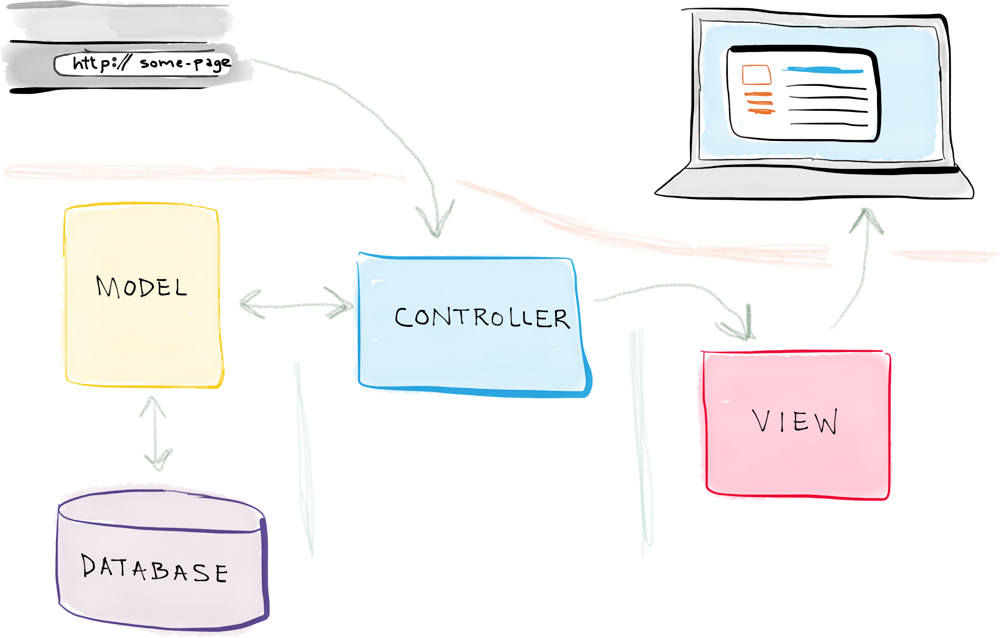
\includegraphics[scale=0.2]{MVC_framework.png}
      \caption{Model View Controller (MVC)}
\end{figure}

We use $CSS$ Scaffolding in Laravel to take care of the views. Buttons and redirections from the user side are implemented in $Javascript$. The models and controllers are written in $PHP$. The specific $MySQL$ database we used it $root$ user's database named $blog$. The website is still hosted on \url{localhost:8000} only.\\
\\
From our modelling for this problem, there are two types of users. The admin users will have different interfaces and unlimited access to all entries. From the user management button in the admin user's profile page. All the users information can be modified and deleted. New users can be added on this panel as well.\\
\\

\newpage

\section{Database Design}

\subsection{Entity-Relationship Diagram}
\newpage

\subsection{Entities}

\begin{center}
Users: \quad
\begin{tabular}{|c|c|}
\hline
Attribute & Domain\\
\hline
email & VARCHAR(64)\\
username & VARCHAR(64) \\
password & VARCHAR(64) \\
mobile & INT(8) \\
address & VARCHAR(128) \\
points\_available & INT(3) \\
admin & INT(1) \\
credit\_rating & NUMERIC \\
created\_at & TIMESTAMP \\
\hline
\end{tabular}
\end{center}

\begin{center}
Items: \quad
\begin{tabular}{|c|c|}
\hline
Attribute & Domain\\
\hline
name & VARCHAR(64)\\
avatar & VARCHAR(256) \\
owner & VARCHAR(64) \\
description & TEXT \\
available & VARCHAR(5)\\
created\_at & TIMESTAMP \\
\hline
\end{tabular}
\end{center}

\begin{center}
Posts: \quad
\begin{tabular}{|c|c|}
\hline
Attribute & Domain\\
\hline
item & VARCHAR(64)\\
title & VARCHAR(64) \\
location & VARCHAR(128) \\
description & TEXT \\
start & TIMESTAMP \\
end & TIMESTAMP \\
created\_at & TIMESTAMP \\
\hline
\end{tabular}
\end{center}

\begin{center}
Bids: \quad
\begin{tabular}{|c|c|}
\hline
Attribute & Domain\\
\hline
bidder & VARCHAR(64)\\
post & VARCHAR(64) \\
status & CHAR(7) \\
points & INT(3) \\
created\_at & TIMESTAMP \\
\hline
\end{tabular}
\end{center}

\begin{center}
Loans: \quad
\begin{tabular}{|c|c|}
\hline
Attribute & Domain\\
\hline
bid & VARCHAR(64)\\
post & VARCHAR(64) \\
start & TIMESTAMP \\
end & TIMESTAMP \\
comments & TEXT \\
status & VARCHAR(8) \\
created\_at & TIMESTAMP \\
\hline
\end{tabular}
\end{center}

\subsection{Relational Schema}
CREATE TABLE users (\\
email VARCHAR(64) PRIMARY KEY,\\
username VARCHAR(64) NOT NULL,\\
password VARCHAR(64) NOT NULL,\\
mobile INT NOT NULL,\\
address VARCHAR(128), \\
points\_available INT DEFAULT 500,\\
admin INT DEFAULT 0,\\
credit\_rating NUMERIC CHECK (credit $>=$ 0 AND credit $<=$ 5),\\
created\_at TIMESTAMP DEFAULT CURRENT\_TIMESTAMP\\
);\\\\
CREATE TABLE items (\\
itemid INT AUTO\_INCREMENT PRIMARY KEY,\\
name VARCHAR(64) NOT NULL,\\
avatar VARCHAR(256),\\
owner VARCHAR(256) REFERENCES users(email) ON UPDATE CASCADE ON DELETE CASCADE,\\
description TEXT,\\
available VARCHAR(5) CHECK(available = `TRUE' OR available = `FALSE'),\\
created\_at TIMESTAMP DEFAULT CURRENT\_TIMESTAMP\\
);\\\\
CREATE TABLE posts (\\
postid int AUTO\_INCREMENT PRIMARY KEY,\\
item int REFERENCES items(itemid) ON DELETE CASCADE,\\
start TIMESTAMP NOT NULL DEFAULT CURRENT\_TIMESTAMP,\\
end TIMESTAMP NOT NULL DEFAULT CURRENT\_TIMESTAMP, \\
title VARCHAR(64) NOT NULL,\\
location VARCHAR(128) NOT NULL,\\
description TEXT,\\
created\_at TIMESTAMP DEFAULT CURRENT\_TIMESTAMP,\\
CHECK (start $<$ end)\\
);\\\\
CREATE TABLE bids (\\
bidid INT AUTO\_INCREMENT PRIMARY KEY,\\
bidder INT REFERENCES users(email) ON UPDATE CASCADE ON DELETE CASCADE,\\
post INT REFERENCES posts(postid) ON DELETE CASCADE,\\
points INT NOT NULL,\\
created\_at TIMESTAMP DEFAULT CURRENT\_TIMESTAMP,\\
status CHAR(7) CHECK (status = `SUCCESS' OR status = `FAILURE')\\
);\\\\
CREATE TABLE loans (\\
loanid INT AUTO\_INCREMENT PRIMARY KEY,\\
bid INT REFERENCES bids(bidid) ON DELETE CASCADE,\\
post INT REFERENCES posts(postid) ON DELETE CASCADE,\\
start TIMESTAMP NOT NULL DEFAULT CURRENT\_TIMESTAMP,\\
end TIMESTAMP NOT NULL DEFAULT CURRENT\_TIMESTAMP,\\
comments TEXT,\\
created\_at TIMESTAMP DEFAULT CURRENT\_TIMESTAMP,\\
status VARCHAR(8) CHECK (status = `ONLOAN' or status = `RETURNED' or status = `EXPIRED'),\\
CHECK (start $<$ end)\\
);

\subsection{Schema Functions}

\newpage

\section{SQL Queries}

\subsection{Simple Queries}

The following simple query returns all the information about one particular bidding specified by bidid. This is displayed when the bidder wants to edit his own bidding.\\
\\
SELECT * \\
FROM bids\\
WHERE bids.bidid = bidid;\\\\
The following simple query returns all the information about all the items. This is displayed when user accesses the `items' page.\\
SELECT * \\
FROM item i;\\\\
The following simple query returns all the information about one particular post. This is displayed when the poster wants to edit his own post.\\
SELECT * \\
FROM posts \\
WHERE posts.postid = postid;\\\\
The following simple query returns all the information about one user with userid specified. This is displayed when the user visited his `user' page.\\
SELECT * \\
FROM users \\
WHERE users.id = userid;\\\\
The following simple query returns all the information about the posts of a particular user specified by his/her email.\\\\
SELECT * \\
FROM posts p, items i \\
WHERE p.item = i.itemid AND i.owner = email;\\\\
The following simple query returns all the information about the transaction history between two users, i.e. their usernames, bidding points, bidding time.\\\\
SELECT u1.username as owner, u2.username as bidder, b.points, b.updated\_at as time\\
FROM users u1, users u2, bids b, items i, posts p\\
WHERE b.bidder = u2.email AND b.post = p.postid AND p.item = i.itemid AND i.owner = u1.email\\
AND (b.bidder = email OR i.owner = email);

\subsection{Aggregate Queries}
The following aggregate query returns the maximum bidding points for one particular post with postid specified. This is displayed when the poster wants to check the maximum bid made for his post.\\\\
SELECT MAX(b.points)\\
FROM bids b, posts p\\
WHERE b.post = p.postid AND p.postid = postid;

\subsection{Nested Queries}
The following nested query 
SELECT p.postid, p.title, p.description, p.created\_at, i1.avatar \\
FROM posts p, items i1 \\
WHERE p.item = i1.itemid\\
AND p.item NOT IN \\
\strut\hspace*{3ex} (SELECT i.itemid FROM items i WHERE i.owner = email);

\subsection{Queries using INNER JOIN}

\subsection{Queries using EXISTS}

\subsection{Queries using set operations}

\subsection{Insertions, Deletions and Updates}
The following query inserts one bidding record into the bids table.\\\\
INSERT INTO bids (bidder, post, points) VALUES (email, postid, points);\\\\
The following query inserts one loan record into the loans table.\\\\
INSERT INTO loans (bid, post, status) VALUES(bidid, postid, using\_status);\\\\
The following query inserts one item record into the items table.\\\\
INSERT INTO items (description, available, name, owner, avatar) VALUES (description, \\ \strut\hspace*{3ex}available, name, owner, filename);\\\\
The following query inserts one post record into the posts table.\\\\
INSERT INTO posts (item, title, location, description) VALUES (itemid, title, location, \\ \strut\hspace*{3ex}description);\\\\
The following query inserts one unsuccessful bidding record into the bids table.\\\\
INSERT INTO bids (status, bidder, post, points) VALUES (`FAILURE', email, postid, point);\\\\
The following query deletes one bidding record.\\\\
DELETE FROM bids\\
WHERE bids.bidid = bidid;\\\\
The following query deletes one post record.\\\\
DELETE from posts\\
WHERE posts.postid = postid;\\\\
The following query updates the bidding points for one particular bidding.\\\\
UPDATE bids\\
SET bids.points = points\_updated \\
WHERE bids.bidid = bidid;\\\\
The following query sets the bidding status to success\\\\
UPDATE bids\\
SET bids.status = 'SUCCESS'\\
WHERE bids.bidid = bidid;\\
UPDATE users set users.points\_available = users.points\_available + points where users.id = userid;\\\\
The following query updates the loan information to be `returned' after the borrowed item has been returned to the owner.\\\\
UPDATE loans l\\
SET l.status = `RETURNED'\\
WHERE l.loanid = loanid;\\\\
The following query updates the post information of a particular post specified by postid.\\\\
UPDATE posts\\
SET posts.title = title, posts.location = location, posts.description = description\\
WHERE posts.postid = postid;

\subsection{Query using view}
Create a view item\_popularity which contains all the popularity information about the items.\\\\
CREATE VIEW item\_popularity AS\\
SELECT i.itemid as itemid, i.owner as owner, COUNT(*) AS popularity\\
FROM items i, posts p, bids b\\
WHERE i.itemid = p.item AND p.postid = b.post\\
GROUP BY i.itemid, i.owner;\\\\
The following query selects the average popularity of the items posted by each user.\\\\
SELECT u.email, AVERAGE(i.popularity)\\
FROM users u, item\_popularity i\\
WHERE u.email = i.owner\\
GROUP BY u.email;\\\\
The following query selects the average popularity of the items bided by each user.\\\\
SELECT u.email, AVERAGE(i.popularity)\\
FROM users u, item\_popularity i, posts p, bids b, loans l\\
WHERE u.email = b.bidder AND b.bidid = l.bid AND b.post = p.postid AND p.item = i.itemid\\
GROUP BY u.email;\\\\
The following query remove the view created.\\\\
DROP VIEW if exists item\_popularity


\newpage

\section{Web Interface Design}
We aims to have a friendly, easy-to-use interface for our web application. The following sections are about the pages in our web interface.
\subsection{Sign Up Page}
\begin{figure}[h]
      \centering
	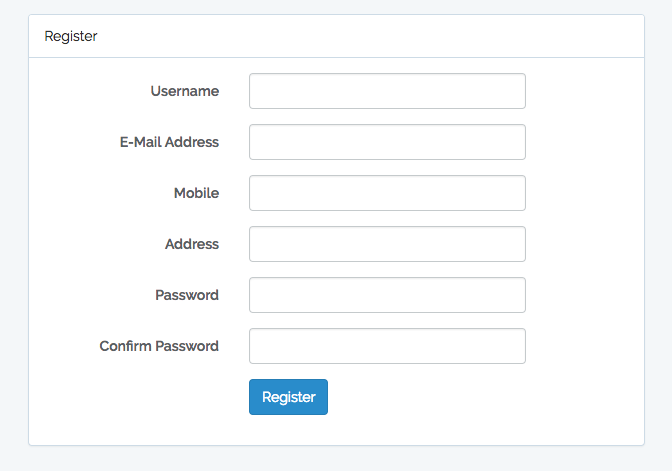
\includegraphics[scale=0.5]{register.png}
      \caption{New User registration page}
\end{figure}
From this page, new users will be able to sign up and enter our system.

\subsection{Log In Page}
Other users will be able to log in via this page.
\begin{figure}[h]
      \centering
	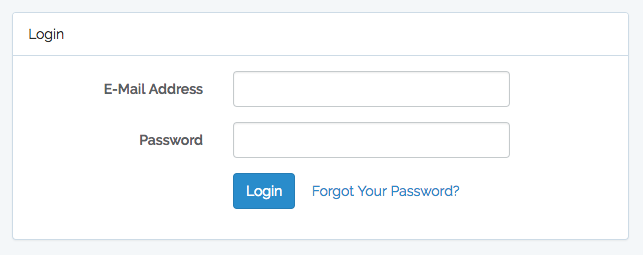
\includegraphics[scale=0.5]{login.png}
      \caption{User login page}
\end{figure}
\newpage

\subsection{Application}
Upon logging in, the user will be directed to his/her dashboard. He can easily see the points available for him or her. Besides that, the items the user owning, the posts he or she has submitted, the posts the user is currently bidding for and the items the user is currently borrowing will be displayed sequentially throughout this the page.\\
\begin{figure}[h]
      \centering
	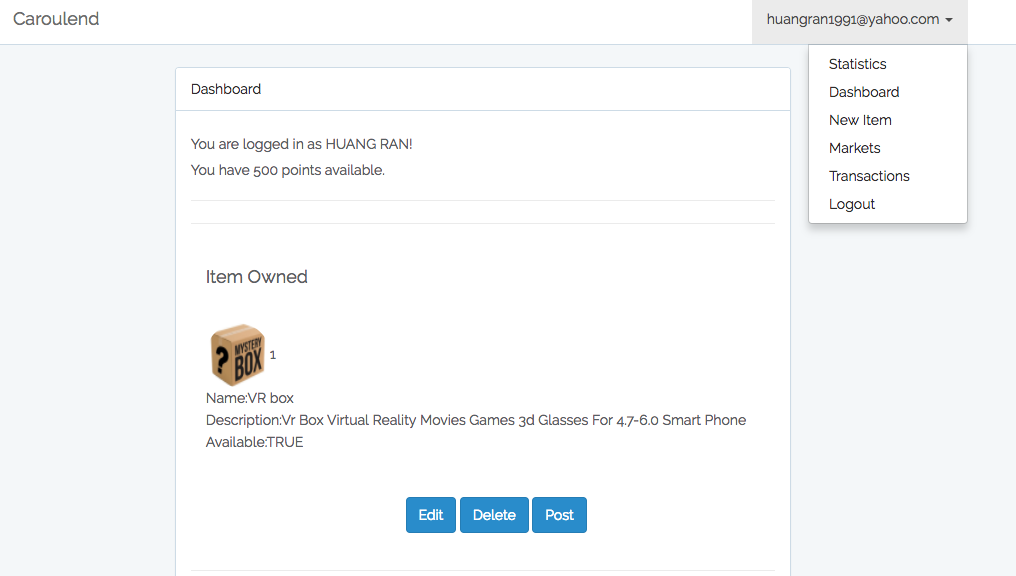
\includegraphics[scale=0.3]{dashboard.png}
      \caption{User login page}
\end{figure}
In addition, from the top right drop down list, the user can go to other pages ranging form his or her using statistics. User can also create new item, go to the posting markets and checkout current transactions and transacting history. This includes the user's posts that are being bid by other users, the user's current lending items and the past transactions.

\subsection{Administration}
There is a special type of user called admin user. They have their admin column equal to 1 and the can have unlimited access to access, delete, update and create any entries in our database. Users are not able to sign up an admin account. The only possible way to become an admin is to update the table in our database directly. Implemented in this way, the administration page is very secure and the current normal users' information are properly protected.
\begin{figure}[h]
      \centering
	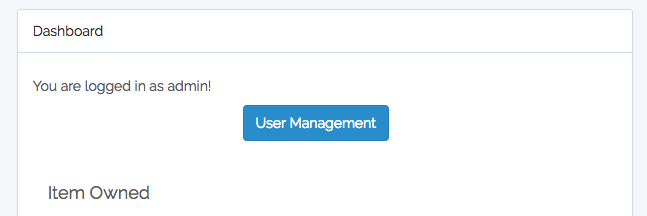
\includegraphics[scale=0.3]{admin.png}
      \caption{User login page}
\end{figure}
As shown in this screen shot, the admin user can access any entries inside this application. If he or she wants to manage the current users, they can do so by clicking the user management button and the user records can be updated, deleted or created on our administration user management panel.

\newpage

\section{Conclusion}

correct way of citing something: \cite{PythonForFinance}

\newpage
\begin{thebibliography}{9}
\bibitem{PythonForFinance} 
Yves Hilpisch,
\textit{Python for Finance}. 
O'Reilly Media, 2015.
 
\bibitem{VarianceReduction} 
Paul Glasserman,
\textit{Monte Carlo methods in financial engineering}.
Springer, 2010.

\bibitem{FiniteDifference} 
Daniel Duffy,
\textit{Finite difference methods in financial engineering: A partial differential equation approach}.
John Wiley\&Sons, 2006.

\bibitem{ContinuityCorrection} 
Mark Broadie, Paul Glasserman, Steven Kou,
\textit{A Continuity Correction for Discrete Barrier Options}.
Mathematical Finance, 1997.

\end{thebibliography}
\end{document}